\section{Ownership Assignment}
\label{section:ownership}


We formulate the last-mile search problem in terms of \textit{locations}, which are searchable entities that 'own' or contain any number of \textit{objects}. Motivated by the way humans tend to recall memories of locations, we designed \emph{GESTALT} to enable users to search for locations using their objects (and optionally their spatial relationships) as the search conditions (i.e. a location that contains <object1, object2, etc.>.)

The objects associated with a given location provide 

..........motivate the use of locations as searchable entities with objects associated to them as the search conditions...........................

After obtaining location and object tags, the next step to enable last-mile search for locations is to determine the ownership relationships between locations and their objects.



We call this problem \textit{Object Ownership Assignment}, and define it as follows:

...........definition latex formatting.................... Given a collection of locations and objects within a region, \emph{Ownership Assignment} seeks to correctly assign each object to its 'parent' location. This amounts to a clustering problem where points (objects) are assigned to centroids (locations) that are known apriori. The objects are not uniformly distributed across locations, and some locations may not have tagged objects associated with them. 


The human eye doesn't see invisible lines on a map. Accordingly, the ownership assignment process is inexact, and objects are 'shared' between locations where appropriate.



The DVBSCAN algorithm Ram et al. proposed in 2010 presents a promising direction to resolve this problem~\cite{Ram2010}, but for simplicity we use DBSCAN and perform a post-processing step to calculate centroids and map them to the nearest location in the dataset. 



\subsection{Dataset}
The experiment design is simple and designed to provide an upper bound for performance on an optimal dataset with no noise (the Swan Valley wineries dataset.) 
The Swan Valley Wineries dataset consists of 31 wineries retrieved from OSM and \~150 objects hand-labeled across 6 of those 31 locations with ground-truth location labels.


\subsection{Method}
1. Use DBSCAN to get the clusters and group objects together, or to the null cluster.
2. Calculate centroids of objects that did cluster (not the null cluster)
3. Calculate probability of object-cluster assignment as 1 - normalized(distance from object to centroid of it's cluster) for non null cluster objects. This adjusts to the density of data rather than using a static parameter (like within x distance). Normalization is done with respect to the real clusters not the null one, since the null cluster has no meaningful centroid and will skew the normalization of the rest of the object-centroid distances.
3a. Set prob = 0.5 for null cluster (as these objects are not relevant or useful in finding locations, since they aren't tied to one, so the search will ignore them anyway)
4. Map the centroids to the nearest location


In step 2: After clustering the objects, we determine the centroid of the object cluster. Given a KD tree constructed from location point coordinates, a nearest neighbor search on the KD tree yields the location nearest to the centroid and it is assigned ownership of that cluster



\subsection{Fuzzy Assignment}
..................TODO NSCH:............ Write up ALGO for fuzzy clustering of objects to locations, where objects can be assigned to multiple locations with some probability p.

Of note, because the human eye can see over property boundaries and other invisible lines on maps, we can accept a small margin of error where objects from neighboring locations might be mislabeled. For example, perhaps there is a large red shed at the back of a location's property that is not visible to the main part of the parent location but is clearly visible to the neighboring location.
There will also exist some objects which plausibly could be seen and remembered by patrons of several locations, for example, a lake or a giant statue. 
This multiple-ownership situation is one of the driving requirements for implementing concept mapping to extract additional discriminatory information between locations based on the geospatial layout of objects.


\subsection{Results}
This section discusses the empirical analysis of the clustering methods tested during the implementation of the Ownership Assignment process. 

RESULTS TABLE HERE.........
\begin{table}[h!]
	\begin{center}
		\begin{tabular}{ |c|c|c|c| } 
			\hline
			Location & Precision & Recall \\
			\hline
			\multirow{7}{4em}{DBSCAN} 
                & $K=1$ & 1 \\ 
			& $K=6$ & 6  \\ 
			& $K=31$ & 31 \\ 
                & $K=1$ & 1 \\ 
			& $K=6$ & 6  \\ 
			& $K=31$ & 31 \\ 
   			& $K=31$ & 31 \\ 
			\hline
		\end{tabular}
		\label{table:clustering}
		\caption{..............}
	\end{center}
\end{table}


\begin{figure*}[ht]
\label{fig:cmeans}        
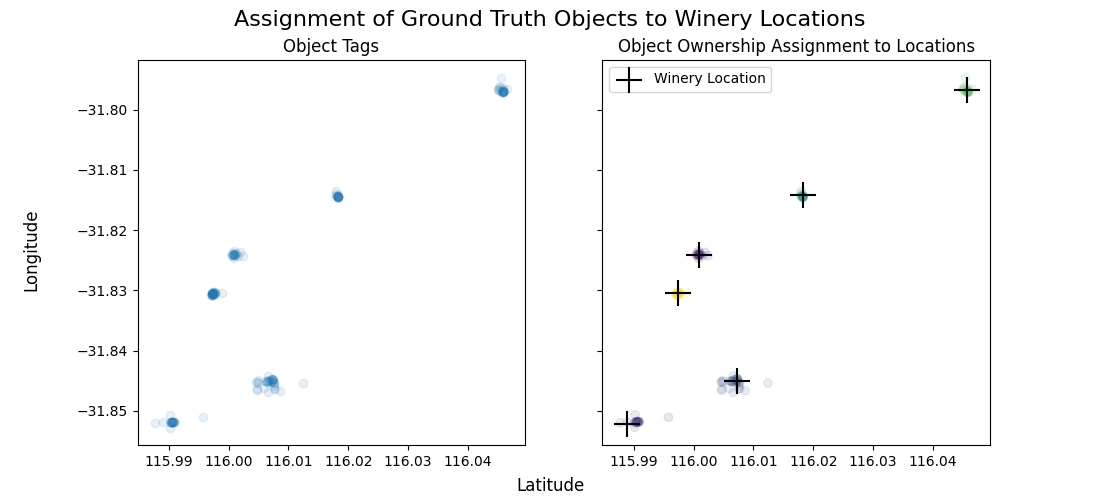
\includegraphics[width=\textwidth]{gestalt_cmeans.png}
\centering
\caption[width=\textwidth]{............}
\end{figure*}


\subsection{Scalability}
The ownership assignment process needs to be unsupervised to enable scaling to millions of object tags. 

- complexity analysis

- present timings/ etc.





%Examining the errors reveals the following insights about each clustering technique. 
%\textbf{When K-Means clusters incorrectly, labels are still correct.} When $K$ exceeds the number of clusters, it fragments the actual clusters. 
%However, in ideal conditions like the Wineries Dataset, where locations are separated, the centroids of these cluster fragments are still closest to the correct location. 
%As a consequence, they are correctly labeled despite being incorrectly clustered. We expect the accuracy will drop when locations are more densely packed. However, when we aim to process all objects and locations in a region concurrently, the number of clusters will likely approach the number of locations, and the issue will be less pronounced. 


%The second, more common (and more challenging approach) formulates an unsupervised learning problem using clustering libraries from \textit{scikit-learn}\footnote{\href{https://pypi.org/project/scikit-learn/}{Scikit-Learn PyPI Repo}}. 

%Ownership assignment is the unsupervised process through which objects are associated with locations. 
%Objects need to be associated with locations in \textit{GESTALT} because for the \textit{concept mapping} process and \textit{search} subsystem to work, they need to know which objects belong to each location.
%For example, assuming two adjacent wineries, a fountain between them would be west of one but east of the other. The mapping will be incorrect unless it is clear which winery it belongs to. 
%Similarly, for search, the underlying idea for \textit{GESTALT} is that people will remember particular objects at locations and use them as clues to find them again. Without an accurate object-to-location assignment, the search functionality will not work. 
 
%The Ownership Assignment process accepts two inputs, a collection of locations with their coordinates and a collection of objects with their coordinates. 
%The process works to assign each object to its parent location. 
%The process ends when objects are mapped to their parent locations. 